%\setcounter{chapter}{5}
\chapter{Normalization verification}
\label{Sect:norm}
\counterwithin{equation}{chapter}

To prove the credibility of an extracted observable, some well-established quantity is commonly used as a reference point. For this purpose one can use already published measurements of this observable, if they exist in the desired kinematic region, but this usually is not the case. Alternatively, one can focus on some quantity, which can be reliably approximated in this kinematic region by a theoretical model or parameterization. 
This auxiliary quantity is then extracted from the analyzed dataset, and the comparison of the measured value with the approximated one allows the reliability of the main result to be judged.

For experiments off a free proton, the elastic cross section usually serves as such a reference quantity as it can be approximated in a wide kinematic region by Peter Bosted parameterization with an excellent accuracy of a few percent, as Ref.~\cite{note_QE_peak}  demonstrates (see App. B there). Therefore an agreement between the auxiliary measured elastic cross section with the parameterized one, if achieved indicates both the correct normalization of the main result and the trustworthy quality of the electron selection.


Meanwhile, for experiments off a deuterium target, the quasi-elastic cross section off nucleons can serve as the corresponding reference quantity. 
However, this observable, if compared with the elastic free proton cross section, is less understood and lacking the same quality of theoretical description~\cite{note_QE_peak}. Nonetheless, several techniques have been developed in this matter with the Bosted parameterization of the deuteron quasi-elastic peak being the most commonly used tool.


%To prove the correct normalization of the obtained results, one is used to carry out a comparison with previously existing data (if they exist in the desired kinematic region) or some theoretical calculations/parameterizations. In the latter case, one usually concentrates on some well-understood and easily-measurable quantities such as the elastic cross section off free proton or quasi-elastic cross section off nucleons in nuclei.

%Nowadays, the elastic cross section off a free proton is well-known over a wide kinematic range, since it has been intensively studied experimentally for decades and eventually almost perfectly described by parameterizations. Meanwhile, the quasi-elastic cross section off nucleons is less understood and lacking the same quality of theoretical description. However, several techniques have been developed on this matter, which includes the Bosted parameterization of the deuteron quasi-elastic peak~\cite{Bosted_fit,Bosted:2007xd}.


Ref.~\cite{note_QE_peak} gives some details on the performance of the Bosted parameterization of the deuteron quasi-elastic peak~\cite{Bosted_fit,Bosted:2007xd} and tests its ability to describe experimental data by comparing the parameterized cross sections with published measurements~\cite{Hanson:1973vf,Rock:1991jy,Rock_SLAC}. This testing, being performed in the $Q^{2}$ range from $\sim$0.3~GeV$^2$ to $\sim$4~GeV$^2$, is of great importance for the current analysis as its $Q^{2}$ coverage falls within this range.


As follows from Ref.~\cite{note_QE_peak}, the Bosted parameterization in its default implementation systematically overestimates the measured integrals under the quasi-elastic peak and the overall description quality gradually decreases from several percent to almost 20\% as $Q^2$ grows from 0.3~GeV$^2$ to 4~GeV$^2$. The default implementation corresponds to the case when the nuclear scaling function is estimated using a PWIA calculation and the Paris deuteron wave function (see Refs.~\cite{Bosted_fit,Bosted:2007xd} for details). 

Meanwhile, as also shown in Ref.~\cite{note_QE_peak}, the Bosted parameterization in its alternative implementation systematically underestimates the corresponding integrals with the description quality gradually increasing from $\sim$15\% to a few percent as $Q^2$ grows from 0.3~GeV$^2$ to 4~GeV$^2$. The alternative implementation corresponds to the case when the nuclear scaling function is estimated according to the parameterization from Ref.~\cite{Bodek:2014pka} and is available with some minor modifications of the source code. 

%However, an alternative way to estimate the scaling function using the parameterization from Ref.~\cite{Bodek:2014pka} is available upon minor modifications of the source code. As shown in Ref.~\cite{note_QE_peak}, the Bosted parameterization in this alternative implementation systematically underestimates the corresponding integrals with the description quality gradually increasing from $\sim$15\% to a few percent as $Q^2$ grows from 0.3~GeV$^2$ to 4~GeV$^2$.

Beside this, Ref.~\cite{note_QE_peak} describes a useful approximation formula for the cross section at the quasi-elastic peak, which came from Durand's theory~\cite{Durand:1961zz}. This formula is of particular interest for this analysis, since it describes very nicely the experimental peak values in the $Q^{2}$ range from $\sim$0.3~GeV$^2$ to $\sim$1.8~GeV$^2$. As shown in Ref.~\cite{note_QE_peak}, the normalization of the cross section distributions of the Bosted parameterization to the values provided by this formula improves the data description quality in this $Q^{2}$ range.




%introduces the mentioned above parameterizations for the deuteron quasi-elastic peak~\cite{Bosted_fit,Bosted:2007xd,Durand:1961zz,Kocevar:1967} and provides the comparison of the parameterized cross sections with two published experimental datasets~\cite{Hanson:1973vf,Rock:1991jy,Rock_SLAC}. In this way the parameterizations’ performance and their ability to describe experimental data are impartially tested and the conclusion on the description reliability is made.

%with two published sets of experimental cross sections



Once we have acquired an impression of the performance and reliability of the parameterizations currently available for the deuteron quasi-elastic peak, let's now estimate the quasi-elastic cross section from the analyzed dataset and then perform its comparison with the cross section approximated by various implementations of the Bosted parameterization. This investigation is carried out in the framework established in Ref.~\cite{note_QE_peak} and therefore, uses the same notations and color codes.


%Once the available parameterization has been tested on the existing data, we have an impression of its performance and ability to describe published experimental measurements. Let's then compare the parameterized quasi-elastic cross section with that obtained from the analyzed dataset. 

To extract the cross section in the region of the quasi-elastic peak, the only particle that should be registered is the scattered electron. With the electron selection being exactly the same as for the double-pion cross section extraction, the quasi-elastic cross section is defined in each $\Delta E' \Delta \theta_{e'}$ bin by \vspace{-1.25em}
\begin{equation}
\frac{d\sigma_{exp}}{d\Omega dE'} = \frac{1}{2\pi} \cdot \frac{\left (\frac{N_{full}}{Q_{full}} - \frac{N_{empty}}{Q_{empty}} \right )}{\Delta E' \Delta(-\cos\theta_{e'}) [\mathcal{L}]} \cdot \frac{N_{gen}}{N_{rec}},\label{eq:my_xsect}
\end{equation}
where $N_{full}$ and $N_{empty}$ are the numbers of selected events inside the $\Delta E' \Delta \theta_{e'}$ bin for runs with deuterium and empty target, respectively. $N_{gen}$ and $N_{rec}$ come from the Monte Carlo simulation and correspond to the numbers of generated and reconstructed quasi-elastic events inside the $\Delta E' \Delta \theta_{e'}$ bin, respectively. The latter were subject to the same electron selection cuts as the experimental events. For the Monte Carlo simulation an event generator based on the measurements from Ref.~\cite{Osipenko:2005gt} was used. The other variables are defined in the context of Eq.~\eqref{expcrossect}.


%\afterpage{\clearpage}
\begin{figure}[htp]
\begin{center}
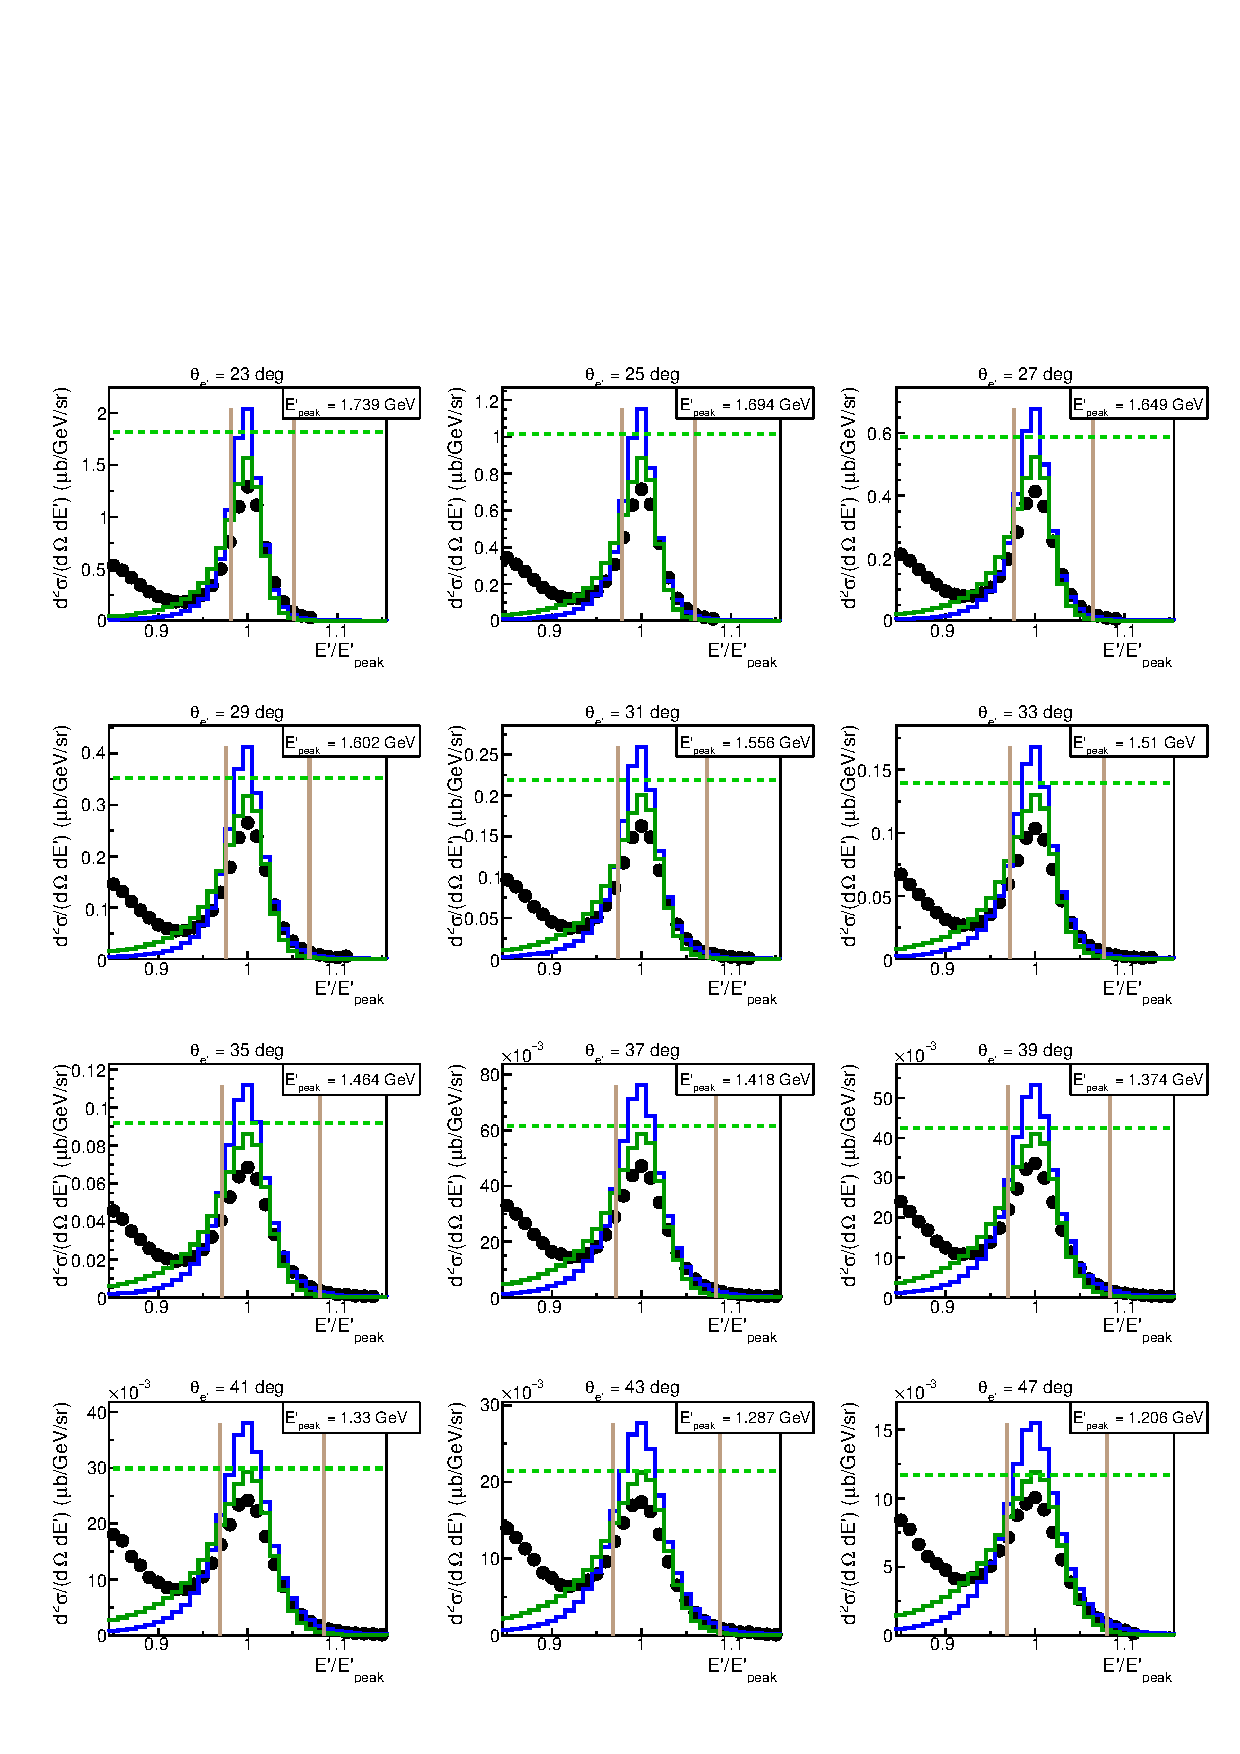
\includegraphics[width=\textwidth]{pictures/normalization/my_xsect_pdf.pdf}
\caption{\small Black symbols correspond to the (radiated) cross section in the region of the quasi-elastic peak extracted from the analyzed dataset according to Eq.~\eqref{eq:my_xsect}. The results of the Bosted parameterization~\cite{Bosted_fit,Bosted:2007xd} are shown by the histograms. The blue histograms correspond to the default method to calculate the nuclear scaling function, while the green histograms to the alternative method. The green horizontal lines correspond to the peak values approximated by the formula described in Ref.~\cite{note_QE_peak}. The vertical lines correspond to the integration limits. } \label{fig:my_QE}
\end{center}
\end{figure}
\begin{table}[htp]
\begin{center}
\caption{\small Ratios of the experimental integrals under the quasi-elastic peak ($\sigma_{exp}$) obtained from the analyzed dataset to those obtained from the Bosted parameterization~\cite{Bosted_fit,Bosted:2007xd} with the nuclear scaling function calculated by the default ($\sigma_{par}^{1}$) and alternative ($\sigma_{par}^{2}$) methods. The index $norm$ means that the parameterization histogram was scaled in a way that its maximum was equal to the prediction of the formula described in Ref.~\cite{note_QE_peak}. The dark-green shade stands for deviations $\leq 5$\%, light-green for 5\%-10\%, and light-red for more than 10\%.   \label{tab:quasi_el_tab_my}}

%\FloatBarrier
 
\begin{tabular}{ 
  !{\vrule width 2pt}
  c!{\vrule width 1pt}
  c!{\vrule width 1pt}
  c!{\vrule width 1pt}
  c!{\vrule width 1pt}
  c!{\vrule width 1pt}
  c!{\vrule width 2pt}
  c!{\vrule width 1pt}
  c!{\vrule width 2pt}
  c!{\vrule width 1pt}
  c!{\vrule width 2pt}
 }
\toprule[2pt]            
\makecell{$\theta_{e'}$,\\ $\!\!\!$deg$\!\!\!$} &\makecell{$Q^{2},$\\ $\!\!\!$GeV$^{2}$$\!\!\!$} & \makecell{$E'_{peak}$,\\ $\!\!\!$GeV$\!\!\!$} &\makecell{Left\\ cut}  & $R$ &\makecell{$\!\!\sigma^{peak}\!\!$,\\ $\mu$b} &$\!\!\sigma_{exp}/\sigma_{par}^{1}\!\!$ &$\!\!\!\sigma_{exp}/\sigma_{\substack{par,\\norm}}^{1}\!\!\!$ &$\!\!\sigma_{exp}/\sigma_{par}^{2}\!\!$ &$\!\!\!\sigma_{exp}/\sigma_{\substack{par,\\norm}}^{2}\!\!\!$\\\Xhline{1pt}
23 &0.56  &1.739 &0.9811 &0.8222   &1.817E0   &\cellcolor{green!20}0.91  &\cellcolor{green!35}1.03  &\cellcolor{red!20}1.13 &\cellcolor{green!35}0.98 \\\Xhline{1pt}
25 &0.65  &1.694 &0.9784 &0.8280   &1.014E0   &\cellcolor{red!20}0.89  &\cellcolor{green!35}1.02  &\cellcolor{green!20}1.10 &\cellcolor{green!35}0.96 \\\Xhline{1pt} 
27 &0.73  &1.649 &0.9761 &0.8325   &5.876E-1  &\cellcolor{red!20}0.87  &\cellcolor{green!35}1.00  &\cellcolor{green!20}1.07 &\cellcolor{green!35}0.95 \\\Xhline{1pt} 
29 &0.82  &1.602 &0.9757 &0.8324   &3.531E-1  &\cellcolor{red!20}0.89  &\cellcolor{green!35}1.04  &\cellcolor{green!20}1.10 &\cellcolor{green!35}0.99 \\\Xhline{1pt} 
31 &0.91  &1.556 &0.9736 &0.8362   &2.188E-1  &\cellcolor{red!20}0.87  &\cellcolor{green!35}1.03  &\cellcolor{green!20}1.07 &\cellcolor{green!35}0.98 \\\Xhline{1pt} 
33 &0.99  &1.51  &0.9722 &0.8384   &1.397E-1  &\cellcolor{red!20}0.85  &\cellcolor{green!35}1.02  &\cellcolor{green!35}1.05 &\cellcolor{green!35}0.97 \\\Xhline{1pt} 
35 &1.08  &1.464 &0.9715 &0.8394   &9.162E-2  &\cellcolor{red!20}0.84  &\cellcolor{green!35}1.02  &\cellcolor{green!35}1.04 &\cellcolor{green!35}0.98 \\\Xhline{1pt} 
37 &1.17  &1.418 &0.9714 &0.8390   &6.167E-2  &\cellcolor{red!20}0.83  &\cellcolor{green!35}1.03  &\cellcolor{green!35}1.04 &\cellcolor{green!35}0.99 \\\Xhline{1pt} 
39 &1.25  &1.374 &0.9694 &0.8427  &4.244E-2  &\cellcolor{red!20}0.83  &\cellcolor{green!35}1.04  &\cellcolor{green!35}1.04 &\cellcolor{green!35}1.00 \\\Xhline{1pt} 
41 &1.33  &1.33  &0.9691 &0.8428  &2.988E-2  &\cellcolor{red!20}0.84  &\cellcolor{green!20}1.07  &\cellcolor{green!35}1.05 &\cellcolor{green!35}1.03 \\\Xhline{1pt}
43 &1.41  &1.287 &0.9686 &0.8436  &2.147E-2  &\cellcolor{red!20}0.83  &\cellcolor{green!20}1.07  &\cellcolor{green!35}1.04 &\cellcolor{green!35}1.03 \\\Xhline{1pt} 
45 &1.49  &1.246 &0.9680 &0.8444  &1.571E-2  &\cellcolor{red!20}0.83  &\cellcolor{green!20}1.09  &\cellcolor{green!35}1.04 &\cellcolor{green!35}1.04 \\ \Xhline{1pt}
47 &1.56  &1.206 &0.9688 &0.8427   &1.171E-2  &\cellcolor{red!20}0.83  &\cellcolor{green!20}1.10  &\cellcolor{green!35}1.04 &\cellcolor{green!35}1.05 \\\bottomrule[2pt]
\end{tabular}
\end{center}
\end{table}%\FloatBarrier
            
              
                 
%Ref.~\cite{Durand:1961zz}      
         


The cross section calculated according to Eq.~\eqref{eq:my_xsect} is shown by the black symbols in Fig.~\ref{fig:my_QE} (note that it is the radiated cross section). The blue and green histograms in this figure correspond to the Bosted parameterization with the default and alternative methods of calculating the nuclear scaling function, respectively. The green horizontal lines correspond to the prediction of the peak value given by the aforementioned approximation formula.  



Since the experimental cross section is radiated, while the parameterized cross section is not, their visual comparison looses informativeness. To judge more definitely the agreement of the measurement with the parameterization, the corresponding integrals under the quasi-elastic peak were compared. The distributions were integrated within the limits shown by the vertical lines in Figs.~\ref{fig:my_QE}. To determine the positions of these limits, the procedure suggested in Ref.~\cite{note_QE_peak} was used.  First, the quasi-elastic peaks in the experimental spectra were fit by Gaussians with polynomial background. Then the values $\mu-\sigma$ and $\mu+3\sigma$ were set as the left and right integration limits, respectively, with $\mu$ and $\sigma$ being the mean value and the standard deviation of the corresponding Gaussian function. The integration limits were chosen to be asymmetrical in order to minimize the inelastic background under the quasi-elastic peak. This procedure of obtaining the integration limits allows to achieve consistency among all plots, since the width of the quasi-elastic peak and its proximity to the inelastic part of the spectrum depend on the kinematics.


%The results of the performed comparison are summarized in Tab.~\ref{tab:quasi_el_tab_my},

The experimental integrated cross sections were divided by the radiative correction factors ($R$), which were calculated in each $\theta_{e'}$ bin according to the Mo\&Tsai approach~\cite{Mo:1968cg}. These correction factors are listed in Tab.~\ref{tab:quasi_el_tab_my} together with the positions of the corresponding left integration limits. The peak cross section values given by the approximation formula are also given there. The last four columns contain the values of the ratio of the experimental integral under the quasi-elastic peak ($\sigma_{exp}$) to that obtained from the Bosted parameterization with the nuclear scaling function calculated by the default ($\sigma_{par}^{1}$) and alternative ($\sigma_{par}^{2}$) methods. The index $norm$ indicates that the parameterization histogram was scaled in a way that its maximum is equal to the prediction of the considered approximation formula. The cells' coloring is the same as for Tab.~1 in Ref.~\cite{note_QE_peak}, i.e. the dark-green shade stands for deviations $\leq 5$\%, light-green for 5\%-10\%, and light-red for more than 10\%.



%for each $\theta_{e'}$ bin


%as well as the values of $E_{peak}$  are listed in Tab.~\ref{tab:quasi_el_tab_my} for each $\theta_{e'}$ bin. 


The ratios of the experimental integrals to the parameterized ones are also shown in Fig.~\ref{fig:my_ratio} as a function of the polar angle of the scattered electron ($\theta_{e'}$). The left side corresponds to the case, when the nuclear scaling function was calculated by the default method (blue symbols), while for the right side it was calculated by the alternative method (green symbols). The top row stands for the unscaled parameterization histograms, while for the bottom row they were scaled to the peak value given by the approximation formula. 



As seen from both Tab.~\ref{tab:quasi_el_tab_my} and Fig.~\ref{fig:my_ratio}, the measured integrals under the quasi-elastic peak were found to be lower than the values given by the Bosted parameterization in its default implementation and their difference increases from $\sim$10\% to $\sim$15\% as $Q^{2}$ grows. The measured integrals were also found to be higher than the values given by the Bosted parameterization in its alternative implementation with the difference decreasing with $Q^{2}$ from $\sim$10\% to $\sim$5\%. Meanwhile, if the parameterization histograms are scaled to the peak values predicted by the formula described in Ref.~\cite{note_QE_peak}, the corresponding ratio stays in the vicinity of unity with a reasonable deviation for both options of scaling function calculation. 

This result is fully consistent with the conclusion made in Ref.~\cite{note_QE_peak} regarding the ability of the Bosted parameterization to describe experimental measurements in this kinematic region. The deviations of the measured integrals from their parameterized values revealed in this analysis and the $Q^{2}$ behavior of those deviations are almost exactly the same as those found in Ref.~\cite{note_QE_peak} for already established measurements.

 




% and 5\%-10\% percent higher than the values given by the Bosted parameterization with the alternative way of nuclear scaling function calculation.


Thus, one can conclude that the quality of agreement between the quasi-elastic cross section estimated in this analysis  with the Bosted parameterization~\cite{Bosted_fit,Bosted:2007xd} is the same as was observed for other published measurements. This, in turn, indicates that in this particular analysis, both the electron selection and overall cross section normalization are under control.

\begin{figure}[htp]
\begin{center}
\begin{framed}
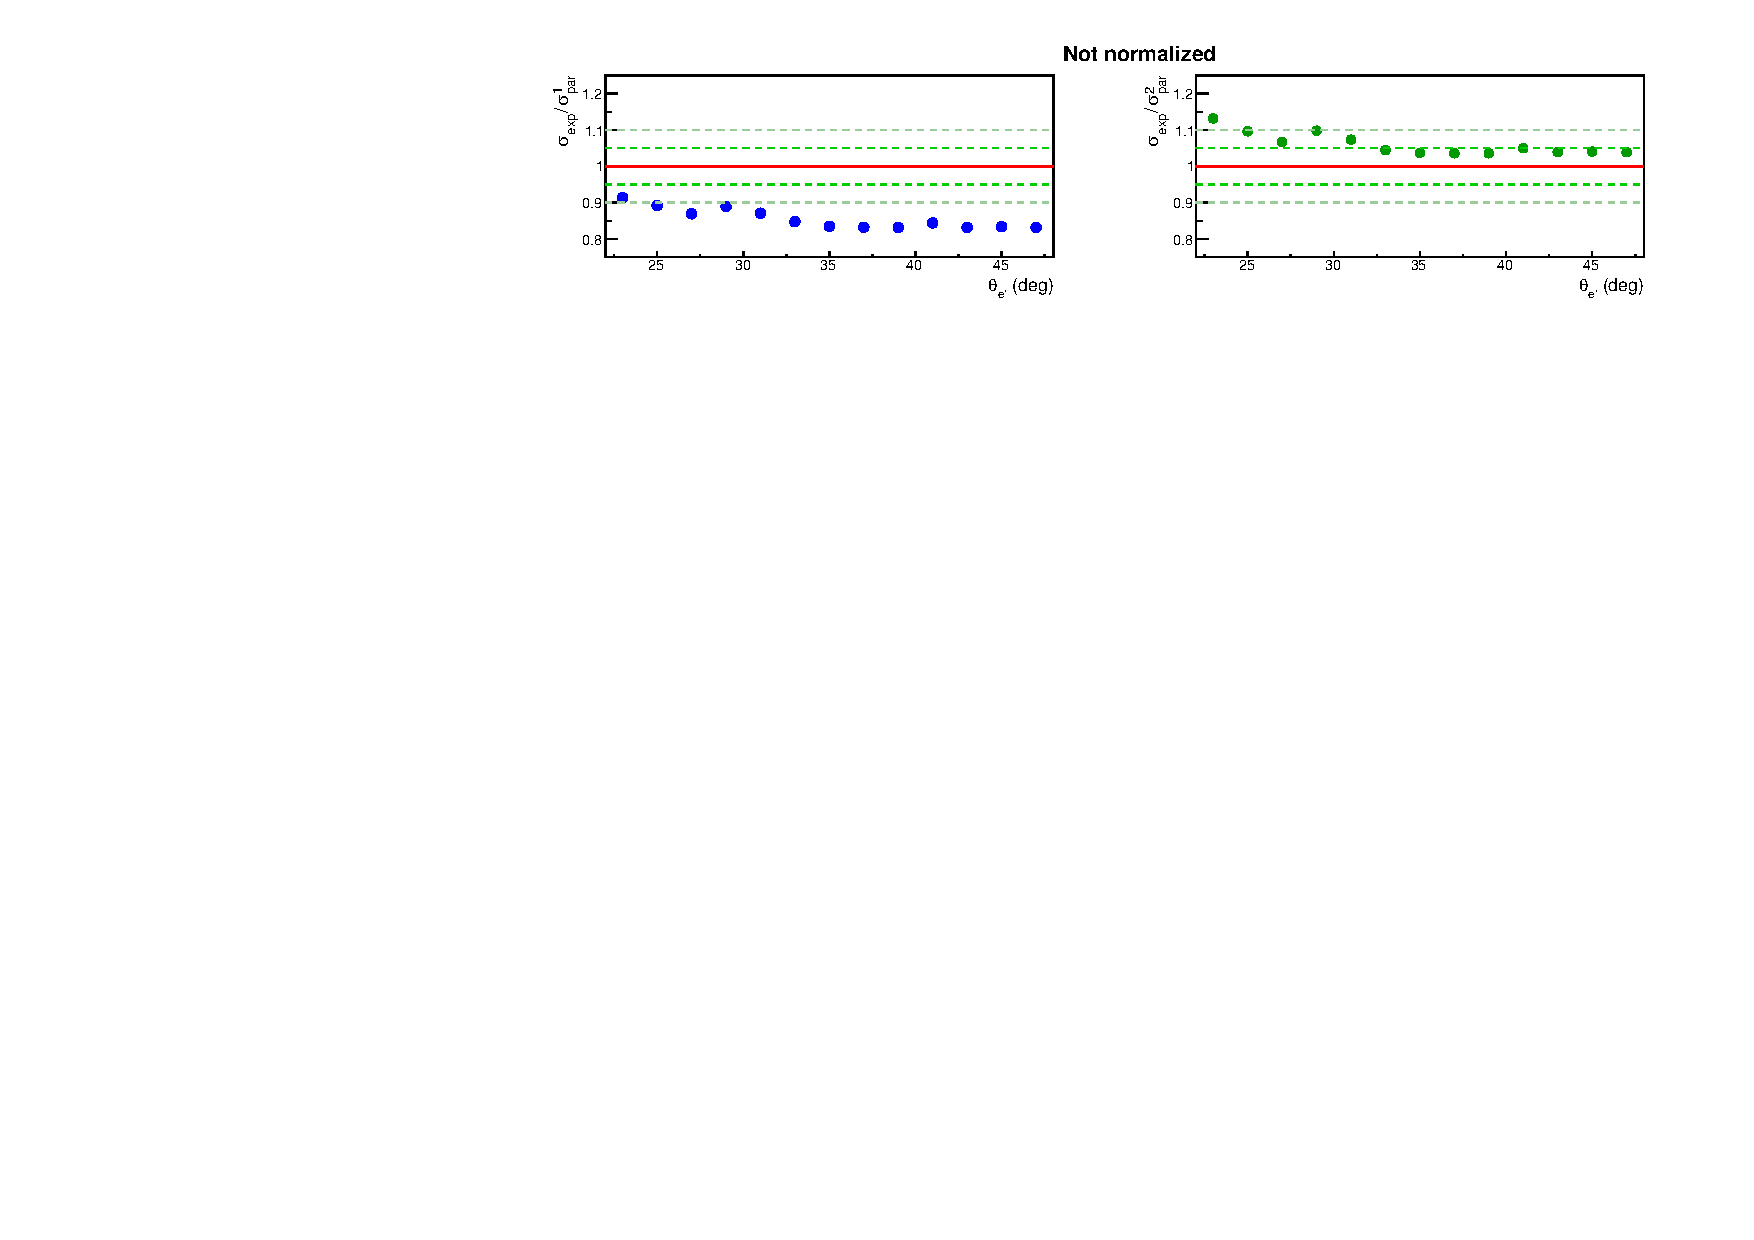
\includegraphics[width=\textwidth]{pictures/normalization/my_ratio_not_norm.pdf}
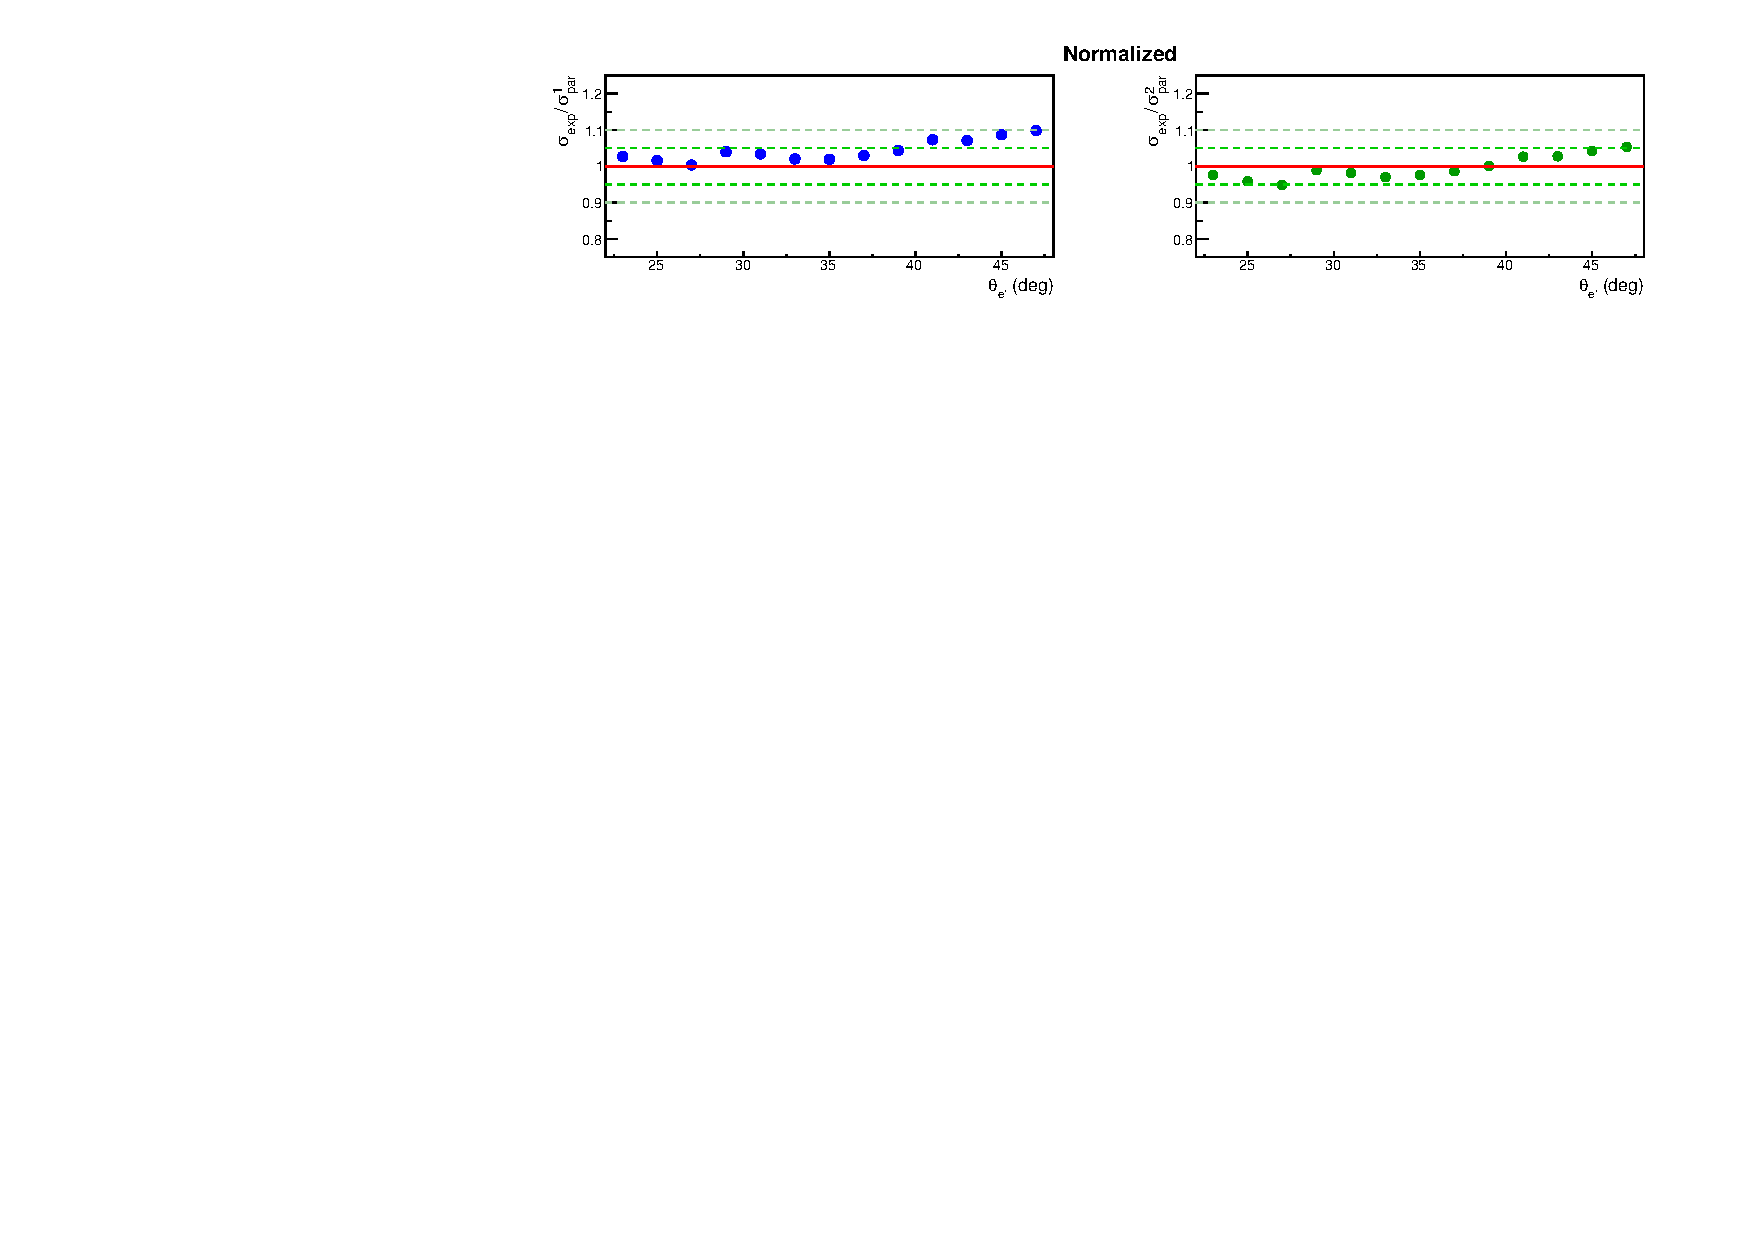
\includegraphics[width=\textwidth]{pictures/normalization/my_ratio_norm.pdf}
\end{framed}
\caption{\small Ratios of the experimental integral under the quasi-elastic peak to the parameterized one as a function of the angle $\theta_{e'}$. The left side corresponds to the case, when the nuclear scaling function was calculated by the default method (blue symbols), while for the right side it was calculated by the alternative method (green symbols). The top row stands for the unscaled parameterized histograms, while for the bottom row, they were scaled to the peak value approximated by the formula described in Ref.~\cite{note_QE_peak}. The red solid line marks the position of unity. The dark-green dashed lines mark the deviation of 5\%, while the light-green ones show the deviation of 10\%.} \label{fig:my_ratio}
\end{center}
\end{figure}


% unscaled Bosted parameterization in its default implementation underestimates the experiment by 10\%-15\%, while for the alternative method it 

% is in good agreement with the experiment with a very slight overestimation.
%\begin{equation}
%\sigma_{exp} (\theta_{e'}) = \frac{1}{R}\cdot \!\!\! \!\!\!\int \limits_{0.97E_{peak}}^{1.2E_{peak}} \frac{d\sigma_{exp}}{d\Omega dE'}\cdot dE' ,
%\end{equation}



%\counterwithin{equation}{section}


%To estimate quantitatively the uncertainty due to normalization and electron identification the following aspects should be considered:

The value of the uncertainty due to normalization and electron identification is then estimated considering the following arguments.

\begin{itemize}

\item as shown in this Section, the quasi-elastic cross section extracted from the current dataset have the same quality of agreement with the Bosted parameterization as other published measurements demonstrate~\cite{note_QE_peak};

\item as follows from Tab.~\ref{tab:quasi_el_tab_my} and Fig.~\ref{fig:my_ratio}, one can achieve a good $\sim$5\% agreement between the measured and parameterized values of the quasi-elastic cross sections when the parameterized distributions are normalized to the peak values approximated by the formula that was proven to describe well the experimental peak cross sections in this kinematic region~\cite{note_QE_peak};

\item as shown in Refs.~\cite{Fed_an_note:2017,Fed_paper_2018}, the elastic cross section off protons estimated from the same ``e1e" run period (as it included both hydrogen and deuterium target runs in the same experimental configuration) agrees within $\sim$3\% with the corresponding Bosted parameterization. The latter, meanwhile, employs the same empirical fit of the nucleon electromagnetic form factors as the Bosted parameterization of the quasi-elastic cross section off deuteron used in the current study~\cite{Bosted:1994tm}.  


% off the free proton estimated in the same kinematic region under the same experimental condition was shown to agree within $\sim$3\% with the corresponding Bosted parameterization~\cite{Fed_an_note:2017,Fed_paper_2018}, which employs the same empirical fit of the nucleon electromagnetic form factors as the Bosted parameterization of the quasi-elastic cross section off deuteron~\cite{Bosted:1994tm}.  


%the study~\cite{Fed_an_note:2017,Fed_paper_2018}, which is the study of double-pion cross sections off the free proton measured in the same kinematic region under the same experimental condition, claims a $\sim$3\% agreement between the measured elastic cross section and its parameterized the Bosted parameterization, which employs the same empirical fit of the nucleon electromagnetic form factors as the Bosted parameterization of the quasi-elastic cross section off deuteron~\cite{Bosted:1994tm}. 

\end{itemize}

Taking these facts into account, a 5\% global uncertainty is assigned to the extracted double-pion cross sections due to potential inaccuracies in the normalization and electron selection.


